\documentclass[tikz,border=3pt]{standalone}
\usepackage[utf8]{inputenc}
\usepackage[T1]{fontenc}
\usepackage{lmodern}
\renewcommand{\familydefault}{\sfdefault}
\usepackage{sansmath}\sansmath
\usepackage{chemfig}
\usepackage{pgfplots}\pgfplotsset{compat=1.18,/pgf/number format/use comma,/pgf/number format/1000 sep={.}}
\usetikzlibrary{arrows.meta,calc,positioning,decorations.pathmorphing,patterns}
% paleta del sitio
\definecolor{nar}{HTML}{E8680C}\definecolor{narc}{HTML}{FFB35C}\definecolor{hielo}{HTML}{FFF3E8}
\definecolor{tinta}{HTML}{1D1D1F}\definecolor{gris}{HTML}{6E6E73}\definecolor{lila}{HTML}{7C5CF0}
\definecolor{azul}{HTML}{2F6FD6}\definecolor{menta}{HTML}{17A673}\definecolor{coral}{HTML}{E8342A}
\begin{document}
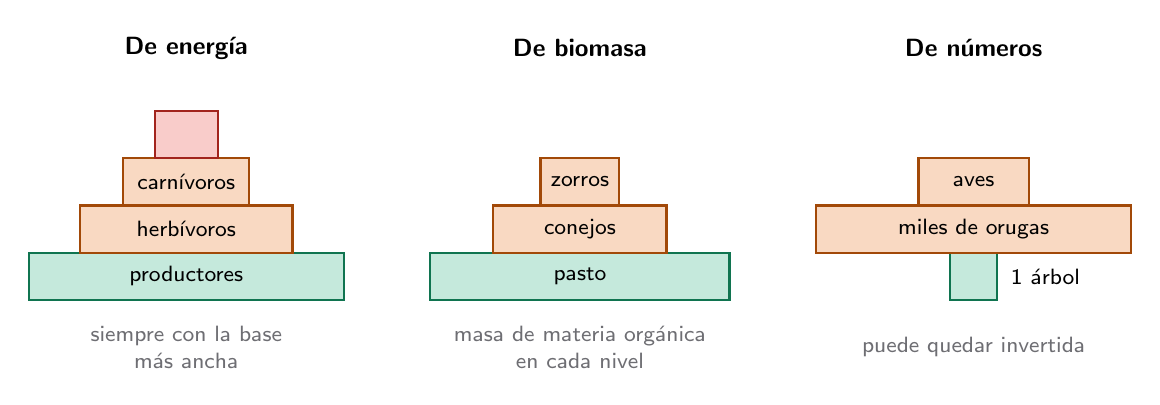
\begin{tikzpicture}[font=\footnotesize]
\tikzset{bar/.style={draw=#1!70!black,fill=#1!25,thick}}
% energía
\begin{scope}[shift={(0,0)}]
\node[font=\small\bfseries] at (0,3.2) {De energía};
\draw[bar=menta] (-2.0,0) rectangle (2.0,0.6) node[pos=0.5] {productores};
\draw[bar=nar] (-1.35,0.6) rectangle (1.35,1.2) node[pos=0.5] {herbívoros};
\draw[bar=nar] (-0.8,1.2) rectangle (0.8,1.8) node[pos=0.5] {carnívoros};
\draw[bar=coral] (-0.4,1.8) rectangle (0.4,2.4);
\node[text=gris,align=center] at (0,-0.6) {siempre con la base\\más ancha};
\end{scope}
% biomasa
\begin{scope}[shift={(5,0)}]
\node[font=\small\bfseries] at (0,3.2) {De biomasa};
\draw[bar=menta] (-1.9,0) rectangle (1.9,0.6) node[pos=0.5] {pasto};
\draw[bar=nar] (-1.1,0.6) rectangle (1.1,1.2) node[pos=0.5] {conejos};
\draw[bar=nar] (-0.5,1.2) rectangle (0.5,1.8) node[pos=0.5] {zorros};
\node[text=gris,align=center] at (0,-0.6) {masa de materia orgánica\\en cada nivel};
\end{scope}
% números
\begin{scope}[shift={(10,0)}]
\node[font=\small\bfseries] at (0,3.2) {De números};
\draw[bar=menta] (-0.3,0) rectangle (0.3,0.6);
\node[anchor=west] at (0.35,0.3) {1 árbol};
\draw[bar=nar] (-2.0,0.6) rectangle (2.0,1.2) node[pos=0.5] {miles de orugas};
\draw[bar=nar] (-0.7,1.2) rectangle (0.7,1.8) node[pos=0.5] {aves};
\node[text=gris,align=center] at (0,-0.6) {puede quedar invertida};
\end{scope}
\end{tikzpicture}
\end{document}
